\documentclass[paper=a4,fontsize=12pt,ngerman]{scrartcl}

\usepackage[utf8]{inputenc} 
\usepackage[T1]{fontenc}
\usepackage{graphicx}
\usepackage[ngerman]{babel}
\usepackage{amsmath}
\usepackage[a4paper,left=25mm,right=25mm,top=25mm,bottom=30mm]{geometry}
\usepackage{parskip}
\usepackage{url}
\usepackage{multirow}
\usepackage{tabularx}
\usepackage{paralist}
\usepackage{xcolor}
\usepackage{amssymb}
\usepackage{enumitem}
\usepackage{listings}

\usepackage[
colorlinks=true,
urlcolor=blue,
linkcolor=green
]{hyperref}
\definecolor{rosa}{HTML}{DF0174}



\newlist{titemize}{itemize}{1}% neue Listenumgebung für Tabellen
\setlist[titemize]{leftmargin=*,nosep,label=-}
% 


\begin{document}
	\pagenumbering{roman}
	\pagestyle{plain}
	
	% Einbinden der Titelseite
	
	\begin{titlepage}
	
	\linespread{1.5}
	
	
\includegraphics[width=\linewidth]{graphics/htw_logo}
	
	\begin{center}
		\large
		\hfill
		\vfill
		\Large{\bfseries{\textcolor{rosa}{Houdini Introduction\\ - \\ Prozedurale Modellierung}}}
		\\
		\large
		von \\
		Jana Koch, Laura Wagner, \\ 
		Nedim Thull, Ali Said, Samantha Maaß
		
	\end{center}
	
	\vfill
	
	
	\vfill
	
	%% {\bfseries{\textcolor{rosa}{}}}\\
	
	
	
	\vfill
\end{titlepage}

	\pagenumbering{arabic}
	\section*{\textcolor{rosa}{Getting started:}}
	\begin{itemize}
		\item Download der Free Test Version von Houdini 18.5.532 from https://sidefx.com/download/.
		\item Registrierung mit Username und E-Mail notwendig.
		\item Anmeldung auf der Webseite bevor Download möglich ist.
		\item Bei der Installation ist es ratsam, neben den bereits markierten Komponenten, direkt die 'SideFX Labs' zu installieren. Dies ist kein muss, spart allerdings Zeit falls man sie später doch benötigt. SideFX Labs ist ein Toolset zur Unterstützung von Aufgaben bei der Erstellung digitaler Inhalte. 
		\item Beim erstmaligen starten von Houdini muss eine Lizenz installiert werden, in unserem Fall die 'free Houdini Apprentice license'.
	\end{itemize}

	\section*{\textcolor{rosa}{Was ist Houdini?}}
		Houdini ist eine 3D-Grafiksoftware, deren Hauptaugenmerk auf der prozeduralen Modellierung liegt. Prozedurale Modellierung beschreibt mit Regeln, wie ein 3D-Objekt erzeugt werden soll. Sie können durch Attribute gesteuert werden und beschreiben Transformationen programmatisch. Dies wird in Houdini mit 'Nodes' realisiert. Sie beschreiben Aktionen die auf die Objekte angewendet werden und können miteinander zu einem 'Network' verknüpft werden. Dadurch lassen sich schnell sehr ähnliche aber einzigartige Objekte schaffen und immer wieder anpassen.  
		
	\section*{\textcolor{rosa}{Interface:}}
	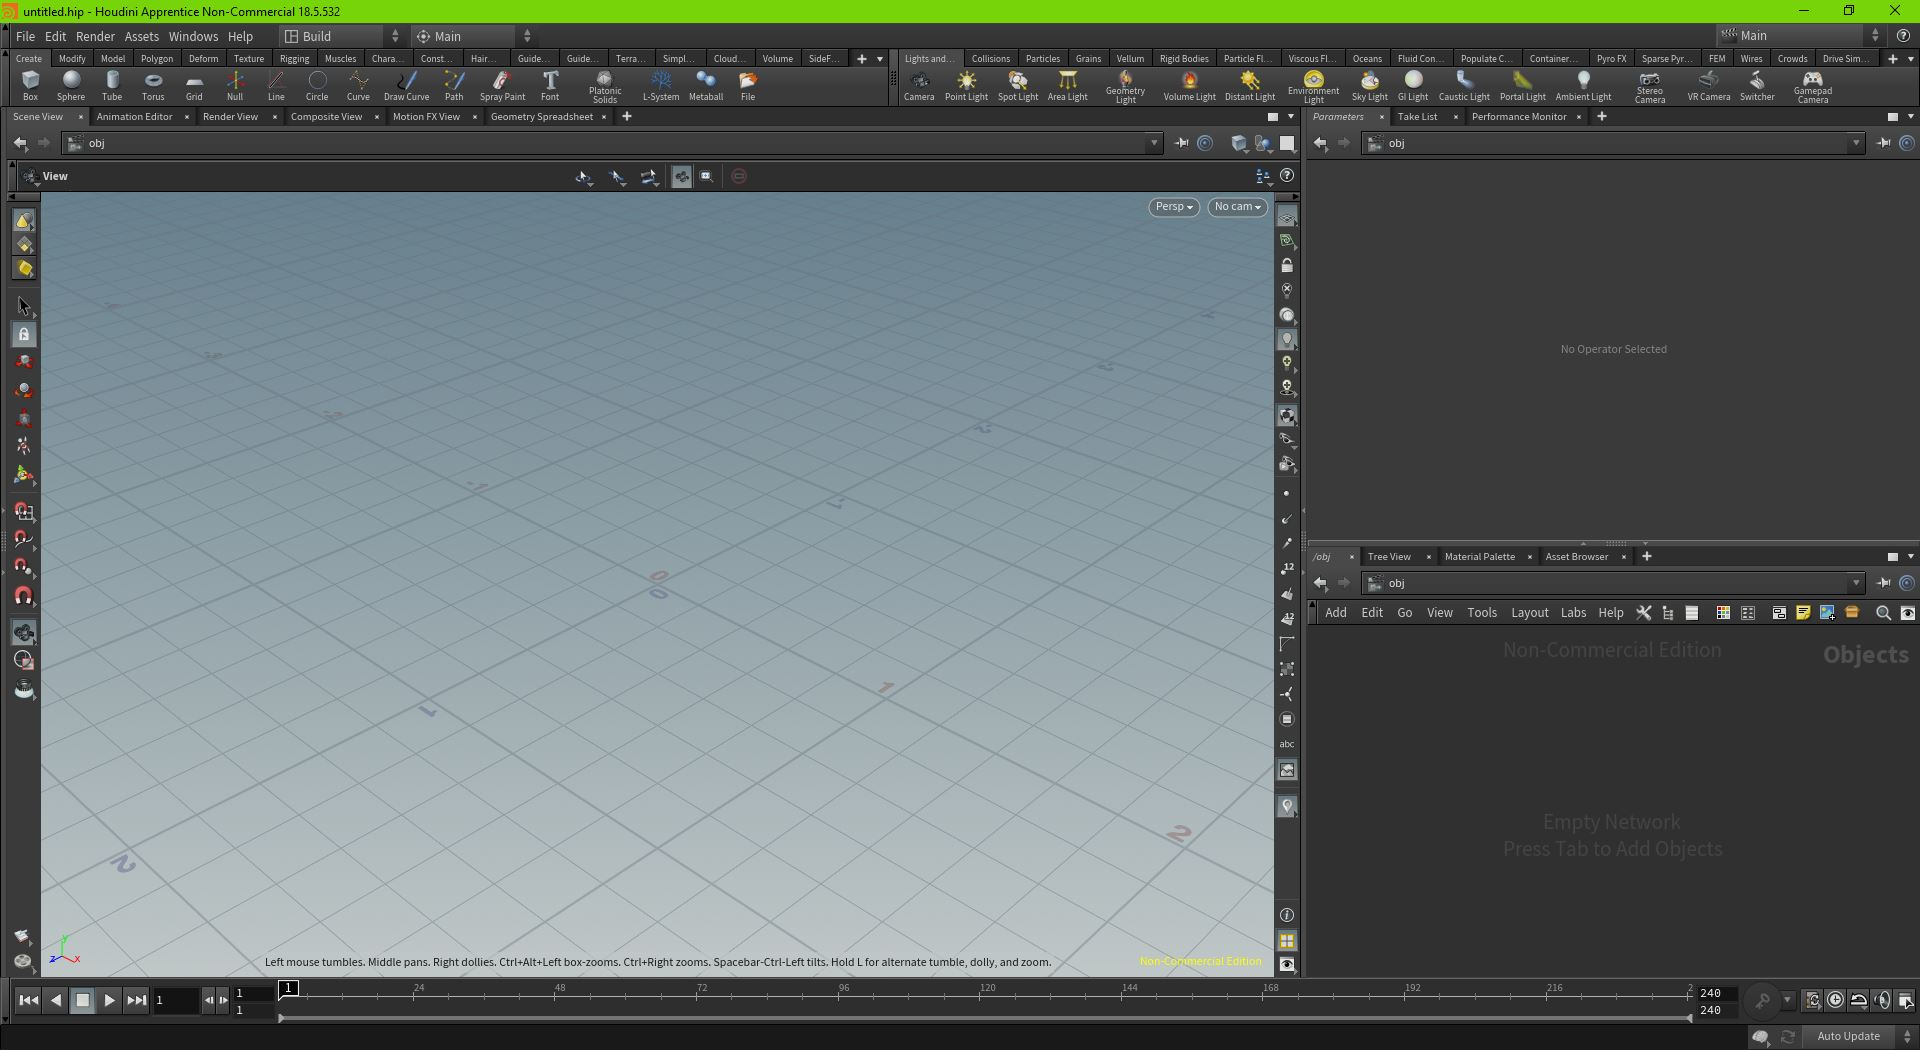
\includegraphics[width=\textwidth]{graphics/Interface.jpg}
	Das Standard-Interface ist in drei Teilbereiche aufgeteilt: 
	\begin{itemize}
		\item Die Scene View, eine 3D Ansicht der aktuellen Szene. (links)
		\item Der Parameter Editor, zum anpassen der Parameter der aktuell ausgewählten Node. (rechts oben)
		\item Der Network Editor, er zeigt alle Nodes des aktuellen Networks, man kann neue anlegen, sie miteinander verbinden und auswählen um die Parameter im Parameter Editor anzupassen. (rechts unten)
	\end{itemize}
	Die Panels können beliebig angepasst, und die Einstellungen gespeichert werden. Die Ansicht in der Scene View kann mit der Maus gesteuert werden: Linke Maustaste zum drehen, mittlere Maustaste zum verschieben und die rechte Maustaste oder das Mausrad zum zoomen. Es macht Sinn sich als erstes mit dem Interface vertraut zu machen, dazu haben wir uns hauptsächlich YouTube-Videos angeschaut. Besonders die 'Houdini isn't scary' - Tutorial Reihe von Nine Between (\url{https://youtu.be/Tsv8UGqDibc}) und die 'Getting started with Houdini' - Reihe von Arise.Works (\url{http://y2u.be/axD1ejlaEBA}) sind sehr zu empfehlen. Allerdings ist die Dokumentation von Houdini und die Tutorials von SideFX selbst sehr gut.(\url{https://www.sidefx.com/docs/houdini/})
	
	\section*{\textcolor{rosa}{Tipps we wish we knew before:}}
	\begin{itemize}
		\item Mit 'Shift + Space + H' wird die Scene View wieder zurückgesetzt.
		\item Der Desktop kann komplett auf Standard zurück gesetzt werden, indem er neu geladen wird.
		\item Nodes können gruppiert, eingefärbt und in Subnetze unterteilt werden.
		\item 'Alle Wege führen nach Rom', aber es gibt immer einen Weg etwas schneller zu machen.
		\item Speichern. Oft.
		\item ESC spammen falls Attribute zu hoch - oder zu niedrig - gesetzt wurden kann einen Progammabsturz verhindern.
		\item Man kann im Parameter Editor die Node nach 'geänderten Parametern' durchsuchen: Lupe > Search All -> 'Parameters with Non-Default Values'
		\item Man kann die Panels auf mehrere Bildschirme verteilen: Pfeil in der rechten oberen Ecke des Panels > Tear off Pane Tab.
	\end{itemize}
		
	\section*{\textcolor{rosa}{Nodes:}}
	
	\subsection*{Attribute:}
 	\subsubsection*{Attribute Blur:}
 	Verwischt Gleitkommaattribute, einschließlich Position, Farbe und Texturkoordinaten, von Punkten in einem Netz, wodurch eine Geometrie effektiv geglättet wird.
 	\begin{itemize}
 		\item Attributes - Welche Attribute verwischt werden sollen, wenn das Feld leer ist, macht die Node nichts
 		\item Method \begin{itemize} 
 			\item Uniform - verwischt gleichmäßig
 			\item Edge Length - verwischt mit Wissen das manche punkte näher sind als andere und behält ihre Abstände bei 
 		\end{itemize}
 		\item Mode	\begin{itemize} 
 			\item Laplacian - jede Iteration hat dieselbe Größe die durch 'step size' definiert wird
 			\item Volume Preserving - Iterationsgrößen werden basierend auf einer Rauschfrequenz ausgewählt, die durch 'Cutoff Frequency' ausgewählt wird
 			\item Custom	Benutzer - kann die Iteration Größen von geraden und ungeraden manuell angeben	
 		\end{itemize}
 		\item Influence Type 
 		\begin{itemize}
 			\item Connectivity - Punkte mischen ihre Attributwerte mit den ihrer Nachbarn, die durch  Mesh-Konnektivität (Verbindungsfähigkeit) erkannt werden
 			\item Proximity - Nachbarn werden durch die nähe bestimmt 
 			\begin{itemize}
 				\item Max - max. Anzahl der Nachbarn
 				\item Proximity Radius - max. Entfernung der Nachbarn
 			\end{itemize}
 		\end{itemize}
 	\end{itemize}
 	
 	\subsubsection*{Attribute create:}
 	Erstellt Attribute der Typen float, Integer, Vector oder String. Falls kein Variablen Name genannt wird, wird der Attribute Name genommen (Groß Buchstaben).\\
 	Value: Stamp ()	gibt eine stamping Variable eine meist danach liegenden Copy Node zurück
 	
 	\subsubsection*{Attribute transfer}
 	Überträgt Scheitelpunkt-, Punkt-, Grundelement- und/oder Detailattribute zwischen zwei Modellen.
 	Die Übertragung funktioniert durch nähe und überträgt Attribute von einem Geometrie Teil auf die nächstliegende Punkte auf einem anderen Geometrieteil. \\
 	unter Attribute kann man die jeweiligen Attribute festlegen. Wenn das Feld leer oder ein Sternchen beinhaltet werden alle verfügbaren Attribute übertragen.
 	\begin{itemize}
 		\item Conditions - gibt an wie Quellattribute kombiniert oder gefiltert werden
 		\item Distance Threshold- gibt die maximale Entfernung von Quellpunkten/Primitiven an, die berücksichtigt werden müssen
 		\item Blend Width - lockert den Distance Treshold und legt optional einen Bereich außerhalb des Distance Treshold fest, in dem der Einfluss der Quellattribute allmählich nachlässt.
 	\end{itemize}
 	
 		\subsubsection*{Attribute Randomize:}
 	Diese Node generiert Zufallswerte, um ein Attribut zu erstellen oder zu ändern. Beispiel Parameter: 
 	\begin{itemize}
 		\item Gruppe – Die Teilmenge der Geometrie, deren Attribut geändert werden soll.
 		\item Attributklasse - Der Elementtyp, für den das durch den Attributnamen angegebene Attribut erstellt oder geändert werden soll.
 		\item Gruppentyp - Der Gruppentyp, den Group angibt.
 	\end{itemize}
 	
 	\subsubsection*{Attribute VOP:}
 	Innerhalb der Node (Doppelklick auf die Node) befindet sich ein VOP Netzwerk. Mit Hilfe von Mathematischen Nodes (z.B. Multiply) lassen sich Attribute Modifizieren.
 	genutzte Nodes:
 	\begin{itemize}
 		\item geometryvopglobal 	alle globalen Variablen für die Attribut-VOP-Netzwerktypen
 		\begin{itemize}
 			\item p - Position des aktuellen Elements
 			\item ptnum (pointnumber) - aktuell verarbeiteter Punkt 
 			\item numpt (number points) - Gesamtanzahl der Punkte
 		\end{itemize}
 		\item divconst - dividiert eingehenden wert durch angegebenen konstanten Wert (Divider)
 		\item divide - Division jedes Eingabewerts durch den nächsten 
 		\item multiply	 - gibt das Produkt der Inputs aus
 		\item inttofloat - wandelt integer zu float um
 		\item vectofloat - wandelt einen Vector zu einer float Zahl um
 		\item floattovec - wandelt eine float Zahl zu einem Vector um
 		\item bind - Bindet die Geometrie an die VEX Funktion um Attribute aufrufe zu können
 		\item ramp- ramp user interface. Der Input ist die Position in der Rampe von dem Wert, welche die Node ausgibt
 		\item turbnoise - berechnet rauschen mit der Fähigkeit, Turbulenzen mit Rauheit und Dämpfung zu berechnen
 		\item displacenml - Verschiebt die Fläche entlang der Flächennormalen um einen bestimmten Betrag
 		\item geometryvopoutput - Platzhalter, um Attribut-VOP-Netzwerktypen herauszuschreiben
 	\end{itemize}
 	
 	\subsubsection*{Attribute wrangle:}
 	entspricht der attribvop Node, aber anstatt des VOP Netzwerks werden hier VEX code Schnipsel genutzt. VEX(Vector Expression Language) ist die Coding Sprache die innerhalb Houdini Verwendet wird und auf C/C++ basiert.
 	Innerhalb des VEXpressions Fenster kann gecodet werden.
 	Verwendeter VEX Code:\\
 	@ repräsentiert Attribute:
 	\begin{itemize}
 		\item @Cd - colour (diffuse) 
 		\item @ptnum - aktuell verarbeiteter Punkt
 		\item @pscale - steuert die Größe (Skalierung) der Punkte
 		\item @elemnum - Nummer des Aktuellen Elements
 		\item @numpt - Gesamtanzahl der Punkte
 		\item @np - die Input Nummer
 		\item @rot - Rotation
 		\item @sc - Skalierung
 		\item @Time - float Time(\$T)
 	\end{itemize}
 	
 	Der Buchstabe vor dem @ repräsentiert den Datentyp: 
 	\begin{itemize}
 		\item f@name - float
 		\item i@name - integer
 	\end{itemize}
 	
 	Funktionen:
 	\begin{itemize}
 		\item addpoint() - int addpoint(int geohandle, int point\_number)\\
 		fügt Punkte einer Geometrie dazu
 		geohandle 	Geometrie, in die der Punkt hinzugefügt werden soll
 		momentan ist der einzig gültige Wert 0 (oder geoself), was die aktuelle Geometrie in der Node bedeutet
 		\item setpointattrib() - int setpointattrib(int geohandle, string name, int point\_num, <type>value, string mode='set')\\
 		Legt ein Punktattribut in einer Geometrie fest:
 		\begin{itemize}
 			\item name - Attribut welches festgelegt werden soll
 			\item point\_num - Nummer des Punktes auf dem das Attribut gesetzt wird
 			\item value - Wert des Attributes
 			\item mode - (Optional)
 			wenn angegeben, steuert wie die Funktion jeden vorhanden Wert im Attribut ändert 
 			'set' überschreibt das Attribut mit dem angegebenen Wert	 	
 		\end{itemize}						
 		
 		\item ch() - float chf(string channel): Wertet einen Channel oder Parameter aus und gibt seinen Wert zurück. Buchstabe nach dem ch gibt Datentyp an:\\ 
 		f -> float\\
 		ramp -> ramp\\
 		float -> chramp(string channel, float ramppos): 
 		wertet einen Ramp Parameter aus und gibt seinen Wert zurück	\\
 		ramppos -> stelle auf der Rampe, die ausgewertet werden soll\\
 		mit ch() erstellte kann man durch klicken von 'Creates spare parameters for each unique call of ch()' anzeigen lassen und bearbeiten. \\
 		\includegraphics*[width=\textwidth]{graphics/attribVOPramp.JPG}\\
 		\item noise() - Es gibt zwei Arten von noise: ändert sich zufällig im gesamtem N-dimensionalen Raum\\
 		nicht periodisches noise: wiederholt sich in einem gegeben Zeitraum\\
 		Die Funktion bestimmt die art:\\
 		vector/float noise(float pos) -> 1D noise\\	
 		vector/float noise(float posx, float posy) -> 2D noise\\
 		vector/float noise(vector pos) -> 3D noise\\
 		vector/float noise(vector4 pos) -> 4D noise\\
 		man bekommt entweder einen Vector aus 3 Zahlen oder eine zufällige float\\
 	\end{itemize}
	
	\subsection*{Digital Assets:}
	
	\subsection*{Group:}
	\subsubsection*{Group Create:}
	Erzeugt Gruppen von Punkten, Primitiven, Kanten oder Scheitelpunkten nach verschiedenen Kriterien.
	\begin{itemize}
		\item Base Group:	
		\begin{itemize}
			\item Base Group - gruppierende Muster, behandelt normale adhoc-Gruppen (keine dauerhafte gruppe, nur unmittelbar zur Lösung eines bestimmten Problems gebildet) Syntax
			\item create ordered - ordnet die Gruppe
		\end{itemize}
		\item Keep in Bounding Regions:
		\begin{itemize}
			\item Enable	- Gruppieren nach begrenzungsvolumen
			\item Bounding Type - Form des begrenzungsvolumen
			\item Size - Größe des begrenzungsvolumen
			\item Center - Mitte des begrenzungsvolumen
			\item Iso - Iso Fläche des Volumens, welche Gruppiert werden soll, Punkte mit niedrigerem Volumenwert werden gruppiert. 
			\item Invert Volume - Volumenwert nicht mehr niedriger, sondern größer
		\end{itemize}
	\end{itemize}

	\subsection*{Import:}
	\subsubsection*{Objekt Merge:}
	Ermöglicht das zusammenführen mehrerer Geometrien. Dadurch reicht es eine Blüte zu erstellen, die wir in allen Blumen Verwenden Können. Wir referenzieren dafür auf die Null-Node, die am Ende jeder Geometrie liegt.\\
	Objekt 1 -> klicke auf 'Open floating operaor Chooser' -> wähle das Objekt (Null-Nodes)
	
	\subsection*{Labs > WorldBuilding > Tree:}
	\subsubsection*{Tree\_Trunk\_Generator:}
	Die Tree Trunk Generator Node ist eine einfache Node, um einen Baumstamm automatisiert erstellen zu können. Hier kann man einstellen, wie lang der Stamm sein soll und wie groß der Radius sein soll.
	\subsubsection*{Tree\_Branch\_Generator:}
	Bei dieser Node ist der Aufbau und die Funktion komplett gleich wie bei dem Tree\_Trunk\_Generator. Was man aber hier anders einstellen kann, ist wie die Gravitation wirken soll. Ob die Äste nach oben, nach unten oder in eine bestimmte Richtung stehen sollen.
	\subsubsection*{Tree\_Leaf\_Generator:}
	Mit Hilfe dieser Node kann man die Punkte einstellen, an denen sich die Blätter am Ast befinden sollen. Man kann einstellen, wo genau die Blätter sein sollen und wie viele es sein sollen. 
	
	\subsection*{Manipulate:}
	\subsubsection*{Bend:}
	Mit der Transformation Node lässt sich das Objekt verschieben, vergrößern, skalieren und rotieren. Bend kann es dazu noch verformen und zum Beispiel biegen und verdrehen. Durch Setzen des Haken bei "Deform in Both Directions" wird die Verformung in beide Richtungen angewendet, welche als Default nur in eine Richtung geht. Um eine Verformung nutzen zu können, muss diese einfach nur aktiviert werden.\\
	Möglichen Verformungen:
	\begin{itemize}
		\item Bend - Biegen
		\item Twist - Verdrehen
		\item Length Scale - strecken(+) und stauchen(-)
		\item Taper- Skalieren am Mittelpunkt
	\end{itemize}
	\subsubsection*{Mountain:}
	Verschiebt Punkte entlang ihrer Normals basierend auf noise. Sie wird häufig verwendet um eine Ebene zufällig zu deformieren. Dies kann auf ein ganzes Objekt oder nur eine bestimmte Gruppe angewendet werden. Zu den wichtigsten Parametern gehören:
	\begin{itemize}
		\item height -> die Höhe der Verschiebung, also wie weit die Punkte von dem eigentlichen Objekt maximal entfernt sein dürfen
		\item Element Size -> Die Distanz zwischen Spitzen der minimalen Noise
		\item roughness -> Je höher der Wert, desto 'Spitzer' wird das Ergebnis.
	\end{itemize}
	\subsubsection*{Transform:}
	Mit der Transform Node, können Objekte beliebig transformiert werden. Dazu gehört das verschieben an eine beliebige Stelle der Szene, sowie das verkleinern, vergrößern oder rotieren in alle Richtungen.
	
	\subsection*{Material:}
	\subsubsection*{Color:}
	Mit der Color-Node kann man ein Objekt einfärben.
	
	\subsection*{NURBS:}
	\subsubsection*{Skin:}
	setzt eine Haut auf eine Form, die eine Oberfläche definiert. Ebenso kann man auch zwischen zwei Oberflächen eine Haut erstellen.\\ 
	Die Anzahl der eingehenden Objekte definiert dabei die Skinning-Methode. Bei nur einem Objekt wird 'Linear-skinning' verwendet, welches eine Haut über Querschnitte zieht. Bei mehreren eingehenden Objekt wird 'Vilineares Skinning' durchgeführt, welches eine Haut zwischen den Objekten zieht.
	
	\subsection*{Particle:}
	\subsubsection*{Scatter:}
	Diese Node verteilt neue Punkte in einem ungefähr gleichförmigen Muster über die Oberfläche und versucht optional, Klumpen und Löcher zu begrenzen. Bei Volumenprimitiven streut Scatter Punkte durch das Volumen mit einer Dichte proportional zum Feldwert (wobei negative Werte eine Wahrscheinlichkeit von Null ergeben).
	
	\subsection*{Polygon:}
	\subsubsection*{Add:}
	Mit add kann man entweder Punkte oder ein Polygon erstellen, oder man fügt Punkte/Polygone einem Input hinzu.\\
	Points:
	\begin{itemize}
		\item Number of Points - Anzahl der Punkte
		\item PointX - die drei Felder entsprechen den x,y,z coordinaten
		\item w - weight (Gewicht), wenn die Punkte später zu einer spline (NURBS or Bezier) werden, beeinflusst das Gewicht die Form und kann dazu führen das sie rational wird
	\end{itemize}
	\includegraphics*[width=\textwidth]{graphics/add.JPG}
	\subsubsection*{Boolean:}
	Kombiniert entweder zwei Objekte mit Boolean Operatoren oder findet ihre Schnittlinie.\\
	
	Set	Treat As Solid -> Festes Objekt\\
	Surface -> Fläche ohne innen und Außenseite\\
	Funktionen:
	\begin{itemize}
		\item Set A -> Solid, Set B -> Solid
		\begin{itemize}
			\item Union - neues Festes Objekt mit dem Volumen von beiden gegebenen Objekten
			\item intersect - neues Festes Objekt mit dem gemeinsam genutzten Volumen der gegebenen Objekte
			\item substract - entfernt das geteilte Volumen von einem oder beiden gegebenen Objekten
			\item shatter - Kombination aus Intersect und Subtract: schneidet entlang der Schnittstellen, um neue Objekte zu erstellen
			\item seam - gibt Polylinien aus, an denen sich die Oberflächen schneiden
		\end{itemize}
		
		\item Set A -> Solid, Set B -> surface
		\begin{itemize}
			\item Union - kombiniert ein festes Objekt mit doppelten Wänden um teile der Fläche außerhalb des Volumens des Festen Objekts herum
			\item intersect - schneidet alle Parts der Fläche weg die außerhalb des festen Objekts liegen
			\item substract - beim Subtrahieren einer Fläche von einem festen Objekt entstehen doppelwandige schnitte im festen Objekt, wo er die Objekte schneidet
			\item shatter - Kombination aus Intersect und Subtract: schneidet die Schnittpunkte in eine neue Form
			\item seam - gibt Polylinien aus, wo die Fläche den Festen Objekt schneidet
		\end{itemize}
		\item Set A -> surface, Set B -> Solid
		\begin{itemize}
			\item Union - kombiniert zusammentreffende Flächen und deren schneidende Teile der beiden Flächen
			\item intersect - behält nur zusammentreffende Flächen
			\item substract - entfernt zusammentreffende Flächen und erstellt doppelseitige schnitte entlang der Schnittpunkte
			\item shatter - Kombination aus Intersect und Subtract:  schneidet Schnittpunkte heraus und behält zusammentreffende Flächen 
			\item seam - gibt Polygone für zusammentreffende Flächen und Polylinien an den Schnittpunkten aus 
		\end{itemize}
		\item custom	- Bei Festen Objekten mit überlappenden oder konzentrischen Flächen kann man Custom nutzen, um einen Bereich an einer gewissen tiefe auszuschneiden
		\item detect	- durchläuft die ersten Geometrien und fügt optionale Gruppen und/oder Attribute hinzu, die die sich schneidende Polygone enthalten.
	\end{itemize}
	\subsubsection*{Facet:}
	Mit Facet kann man die Geometrie in Etappen ändern. Man kann z.B. Oberflächennormalen berechnen, bevor man Punkte, die von verschiedenen Polygonen geteilt werden, eindeutig macht. Das führt zum ungewöhnlichen Ergebnis einer glatten Schattierung und eines eindeutigen Punkts, da die Normalen berechnet werden, während die Punkte noch geteilt werden. 
	\subsubsection*{Normal:}
	Dieser Knoten berechnet Punkt-, Scheitelpunkt-, Grundelement- oder Detailnormalen unter Verwendung eines genaueren Ansatzes als der Facettenknoten oder der Scheitelpunktknoten. Wird der 'Cusp Angle' auf 0 gesetzt, können die Kanten eckig gemacht werden.
	\subsubsection*{PolyBevel:}
	Polybevel fügt Verrundungspolygone zwischen Kanten und in Ecken ein, mit großer Kontrolle über die Form der Verrundung, durch die Anzahl an Divisions und der Distanz. Diese Node kann sehr komplexe Eingaben verarbeiten und ignoriert nicht-beitragende Kanten.
	\subsubsection*{PolyExtrude:}
	Mit Poly Extrude kann man Flächen und Kanten 'herausziehen', um neue Spalten/Blätter von Polygonen zu erstellen. Man kann die Extrusion vergrößern oder verkleinern (Einsatz/Anfang) und verdrehen. 
	\subsubsection*{PolyReduce:}
	Polyreduce bietet eine sehr schnelle, hochpräzise Reduktion, während Form, Texturen, Attribute und Quad-Topologie der Eingabe so weit wie möglich beibehalten werden. Es hat mehrere Funktionen, mit denen Sie kontrollieren können, wo der Knoten verkleinert und umgeformt wird:
	\begin{itemize}
		\item Sie können verhindern, dass der Knoten ungeteilte Kanten im 3D- und UV- Raum verschiebt.
		\item Sie können Punkte und/oder Kanten angeben, die beibehalten werden sollen. 
		\item Sie können ein Attribut in Bereichen zeichnen, in denen Sie mehr Dichte beibehalten möchten. 
		\item Sie können Polygone basierend auf der Sichtbarkeit von bestimmten Ansichtspunkten aus beibehalten. 
	\end{itemize}
	\subsubsection*{Remesh:}
	Rekreiert die Fläche mit 'hochwertigen' (fast gleichseitigen) Dreiecken (hochwertiges dreiecksnetz = alle Winkel so nah wie möglich an 60 Grad). Dabei wird versucht in jedem Dreieck den kleinsten Winkel zu maximieren.
	Es gibt zwei Arten von Remeshing:
	\begin{itemize}
		\item Uniform - versucht Kantenlängen auszugleichen und erstellt so gleichgroße Dreiecke
		\item Adaptive - passt die Größe den Bereichen an und erstellt größere Dreiecke in breiten Bereichen und kleinere Dreiecke in detaillierten Bereichen
	\end{itemize}
	\begin{itemize}
		\item Iterations - die Qualität des Netzes, Im Normalfall ist die maximal nützliche Anzahl 3 bis 4
		\item Recompute Normals - berechnet neue normals für das generierte netz
		\item Smoothing - grad der Glättung
	\end{itemize}
	
	\subsubsection*{Subdivide:}
	nimmt eine Polygon Fläche und teilt jeden Bereich, um die Fläche zu glätten.
	\begin{itemize}
		\item Groups - Alle Polygone in der linken Eingabe, werden verwendet, um das zu unterteilende Polygonnetz zu bestimmen.
		\item Creases - Elemente der rechten Eingabe werden als Knicke genutzt.
		\item Depth - Wie viele Iterationen zu unterteilen sind
	\end{itemize}
	
	\subsection*{Primitive:}
	\subsubsection*{Box:}
	Ein einfaches/-r Quadrat/Quader.
	\subsubsection*{Grid:}
	Erstellt eine flache Ebene, die aus einem Netz, Bezier- und NURBS-Flächen oder mehreren Linien mit offenen Polygonen bestehen kann. Häufig genutzte Parameter:
		\begin{itemize}
			\item Size - Breite und Höhe des Rasters.
			\item Rows - Anzahl der Reihen im Raster oder Rumpf. 
			\item Column - Anzahl der Spalten im Raster oder Rumpf.
		\end{itemize}
	\subsubsection*{Line:}
	Erstellt ein Polygon oder eine Linie.
	\begin{itemize}
		\item Primitive Type - Geometrie Typ  
		\item Origin - Start der Linie
		\item Direction - Richtung der Linie
		\item Length - Länge der Linie
		\item Points - Anzahl der Punkte mit der die Linie erstellt wird
	\end{itemize}
	\subsubsection*{L-System:}
	Das Lindenmeyer-System ist ein Algorithmus zum Umschreiben von Zeichenfolgen. Einfach gesagt ersetzt der Algorithmus nach einer bestimmten Regel Zeichen durch andere Zeichen bzw. Zeichenketten.
	Durch Verwendung von Iterationen, wobei die Ergebnisse zur Grundlage der nächsten Iteration werden, kann man ein Wachstum darstellen. In unserem Fall nutzen wir sie, um Blumen und deren Verzweigungen am Stängel herzustellen. 
	\begin{itemize}
		\item GEOMETRY:
		\begin{itemize}
			\item Type - Skeleton = einfache Linien; Tubes = Röhren
			\item Generation - gibt an wie viele Generationen im Falle einer Iteration durchlaufen werden
			\item Apply Colour - durch setzen werden die Farben der eingefügten Objekte übernommen
		\end{itemize}
		\item TUBES:
		\begin{itemize}
			\item rows \& cols - gibt Anzahl der Reihen und Spalten des 'netztes' der Röhren an
			\item Tension - wie gerade die Röhren zu ihrem Zielpunkt gehen
			\item Thickness - breite der Röhre
		\end{itemize}
		\item RULES:		
		\begin{itemize}
			\item Premise - Ausgangszustand des L-Systems - Generation 0
			\item Rule\#  - Regeln/Formeln die den Verlauf des L-Systems beschreiben
		\end{itemize}
		Befehle die genutzt werden:  
		\begin{itemize}
			\item $[]$ - erstellt ein neuen Branch
			\item \{\} - erstellt ein Polygon
			\item ABCD - Variablen die für die einzelnen Regeln stehen
			\item JKM - verweist auf die Objekte bzw. die Eingänge 
			\item F(a) - erstellt eine einfache Linie. Man kann sie zusätzlich durch einen Wert in einer folge Klammer verkürzen/verlängern
			\item .  - Polygon Vertex (Vertex = Ecke eines Polygons)
			\item !(s) - Multipliziert momentane breite mit s. In unserem Fall bewirkt es, das die röhren immer schmaler werden
			\item \&(a) - nach oben kippen um a grad
			\item \^(a) - nach unten kippen um a grad
			\item "(s) - multipliziert bzw. skaliert die momentane Branch länge mit s
			\item /(a) - dreht im Uhrzeigersinn a grad
			\item -(a) - rotiert nach links um a grad
			\item +(a) - rotiert nach rechts um a grad
		\end{itemize}
	\end{itemize}
	\subsubsection*{Sphere:}
	Sphere ist eine einfache Node, die ein Kugel Objekt erstellt. Man kann bei dem Primitive Type einstellen, welche Oberfläche die Kugel haben soll. Man kann den Radius bestimmen, die Frequenz und auch wie die Höhe und Breite der Kugel, dadurch kann man zum Beispiel auch Ovale formen. 
	\subsubsection*{Tube:}
	Ein Tube ist ein einfacher Kegel. Häufig genutzte Parameter: 
	 	\begin{itemize}
	 		\item Radius - Radius der Tube. 
	 		\item Radius Scale - Einheitlicher Maßstab für den Radius. 
	 		\item Height - Die Höhe der Tube. 
	 	\end{itemize} 
	
	\subsection*{Utility:}
	\subsubsection*{Convert:}
	Konvertiert eine Geometrie Art zu einer anderen Geometrie Art
	\begin{itemize}
		\item From Type - Welche Art die Geometrie hat
		\item Convert To- Welche Art die Geometrie danach haben soll
	\end{itemize}
	Division per Span
	\begin{itemize}
		\item Genaue Anzahl der Punkte
		\item U- Punktdichte in U Richtung
		\item V - Punktdichte in V Richtung
		\item U Order- Spline-Reihenfolge von Kurven und Flächen in U
		\item V Order - Spline-Reihenfolge von Kurven und Flächen in V
		\item Interpolate Through Hulls - Die Form der Geometrie wird übernommen, deaktiviert U \& V
	\end{itemize}
	\subsubsection*{Copy Stamp:}
	Copy besitzt zwei Hauptaufgaben:
	- mehrere Kopien einer Geometrie erstellen
	- Kopiert die erste Geometrie an Punkte der Zweiten Geometrie
	Die einzelnen Kopien können zusätzlich mit COPY transformiert werden. 
	Durch STAMP -> Stamp Inputs können Variablen für jede Kopie weitergeführt werden. 
	\subsubsection*{Copy to Points:}
	Wie der Name schon sagt, kopiert es ein Objekt (erster Input) an übergebene Punkte (zweiter Input). Wird in unserem Fall innerhalb einer Schleife genutzt
	\subsubsection*{Merge:}
	Diese Node führt die Geometries aus seinen Eingaben zu einem einzigen Geometriestrom zusammen, den Sie dann durch andere Nodes senden können. Sie fügt quasi zwei Objekte zusammen. Die Merge-SOP wendet alle eingehenden Attribute auf die gesamte Eingabegeometrie an. Jede Eingabegeometrie kann ihren eigenen Satz von Attributen haben.
	\subsubsection*{Mirror:}
	Dupliziert und spiegelt das Objekt. 
	\subsubsection*{Null:}
	Das Null Objekt dient zum einen als Platzhalter. Es kann verwendet werden, um einen Ort im Raum der Scene zu bestimmen oder als 'Betrachtungsobjekt' als Hilfe für die Koordination in der Szene. Seine Parameter ähneln denen von 'Transformieren' und 'Verschiedenes'. Es kann ein Objekt Transformieren und hilft später besser auf das Objekt referenzieren zu können
	\subsubsection*{For Each (begin \& End):}
	For Each beinhaltet zwei Nodes: begin und end. Der Context der Schleife steht in der Input-Node der begin-Node, was in unserem Fall unsere Punkte sind. Die For Each Schleife geht nun jeden Punkt durch und wendet die Nodes die zwischen begin und end liegen auf jeden dieser Punkte an.
	
	\section*{\textcolor{rosa}{Tutorials:}}
	\subsection*{Terrain:}
	 Siehe Word Dokument
	
	\subsection*{Wasser:}
	\begin{minipage}{0.5\textwidth}
		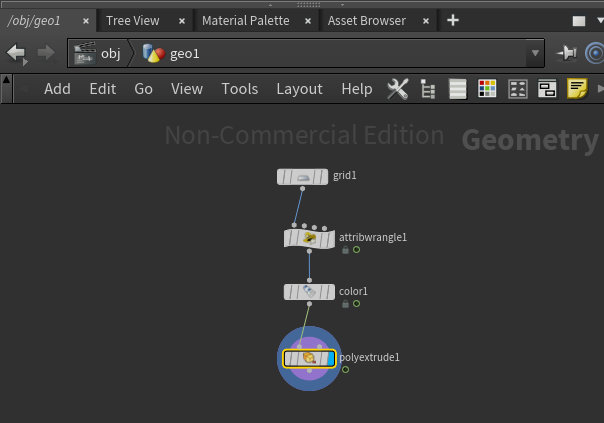
\includegraphics[width=\textwidth]{graphics/wasser_1.png}
	\end{minipage}
	\begin{minipage}{0.5\textwidth}
		Zuerst wird eine Geometry erstellt. In dieser Geometry wird eine Grid-, eine Attribute Wrangle-, eine Color- und eine Poly Extrude-Node benutzt.
	\end{minipage}
	
	\begin{enumerate}
		\item Das Grid wird zuerst gesetzt und es können die Werte von rows und Columns (je mehr desto 'realistischer'), sowie Länge und Breite geändert werden. 
		\item 
		\begin{minipage}{0.5\textwidth}
			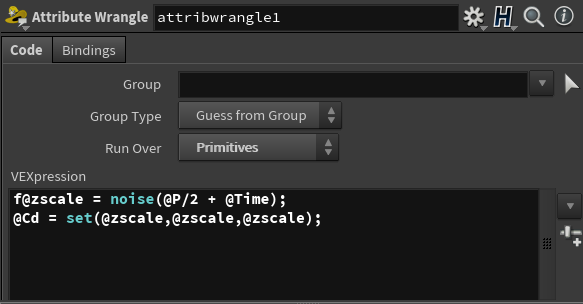
\includegraphics[width=\textwidth]{graphics/wasser_2.png}
		\end{minipage}
		\begin{minipage}{0.5\textwidth}
			Als Zweites kann man die Attribute Wrangle-Node setzen und definiert die Atrribute mit einer 'VEX expression':\\
			Wir benutzen dies hier, um an manchen Stellen auf dem Grid dunklere und hellere Flächen in Abhängigkeit von der Zeit zu setzen, die die Wellen des Wassers darstellen.
		\end{minipage}
		\item 
		\begin{minipage}{0.5\textwidth}
			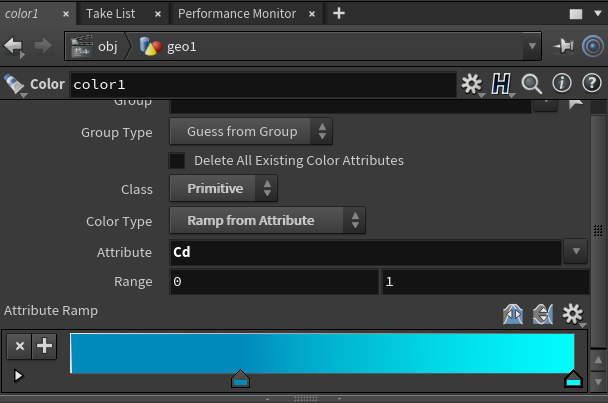
\includegraphics[width=\textwidth]{graphics/wasser_3.png}
		\end{minipage}
		\begin{minipage}{0.5\textwidth}
			Mit Color kann man die gewünschte Farbe angeben, die in diesem Fall Blau ist.\\
		\end{minipage}
		\item 
		\begin{minipage}{0.5\textwidth}
			Als letztes setzt man die Poly Extrude-Node. In dieser Node werden die Werte folgender Maße gesetzt:
		\end{minipage}
		\begin{minipage}{0.5\textwidth}
			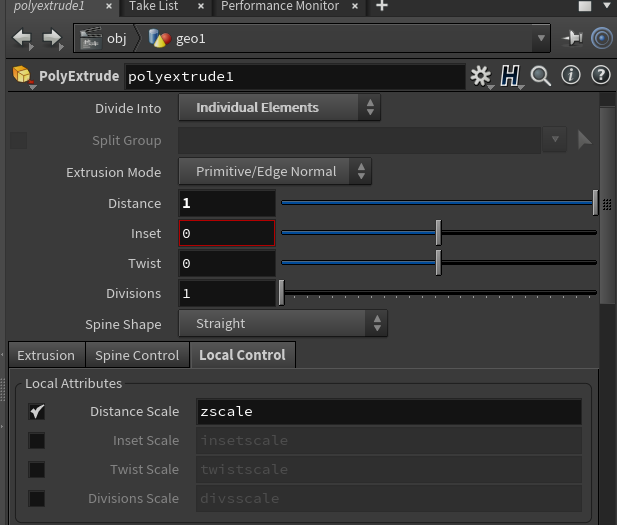
\includegraphics[width=\textwidth]{graphics/wasser_4.png}
		\end{minipage}
	\end{enumerate}
	\begin{minipage}{0.5\textwidth}
			Das Objekt sollte damit so aussehen:
	\end{minipage}
	\begin{minipage}{0.5\textwidth}
		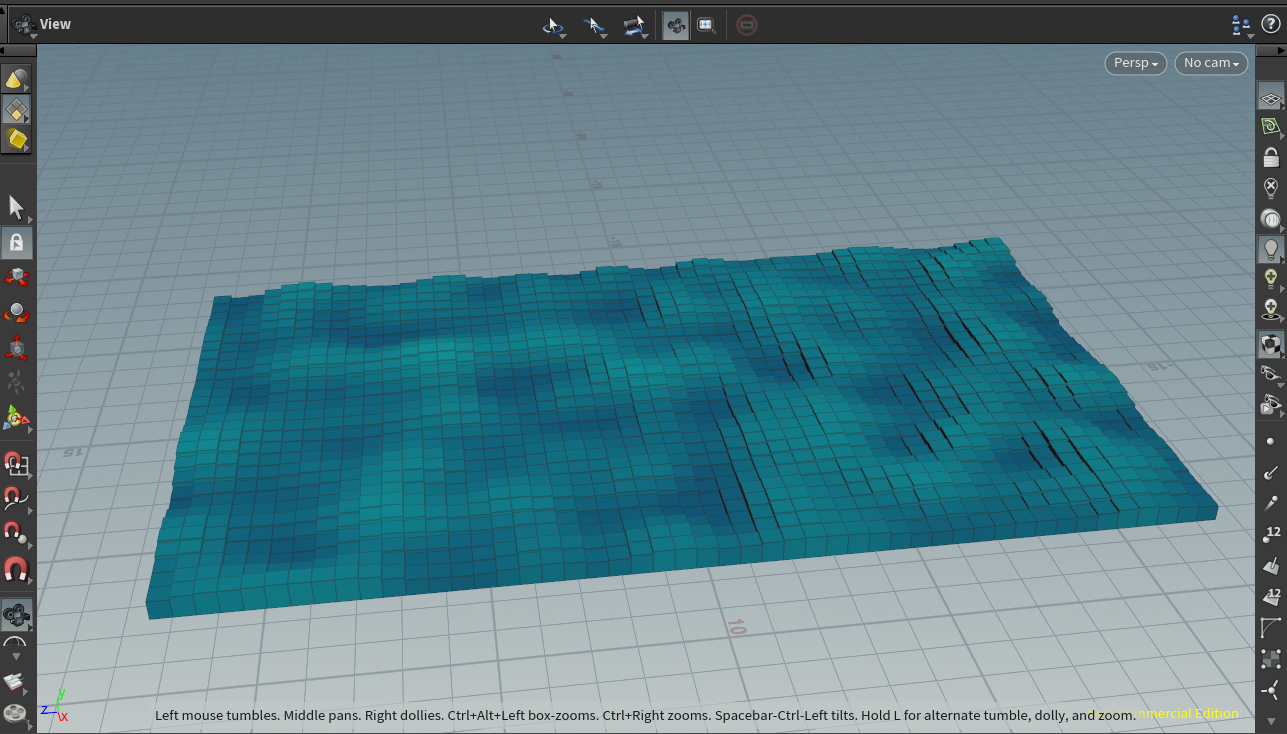
\includegraphics[width=\textwidth]{graphics/wasser_5.png}
	\end{minipage}
	
	\subsection*{Steine:}
	Die Steine bestehen aus einem sehr simplen Aufbau von nur vier Nodes. Eine normale Sphere, die etwas gestaucht wird um die Steine etwas flacher zu gestalten. Diese wird mit einer 'Mountain' Node uneben gemacht und mit einer 'Normal' Node die Kanten eckiger gemacht, um den Low Poly Stil umzusetzen. Anschließend wird die Sphere mit einer 'Color' Node grau eingefärbt.
	
	\subsection*{Gras:}
	Um Gras zu modellieren gibt es wie bei allem viele verschiedene Möglichkeiten. Die einfachste davon ist es das Hair-Tool zu benutzen. Das Hair Tool ist ein eingebautes Houdini-Tool um eigentlich Fell, oder Haare zu generieren. Man kann es jedoch auch benutzen um flächendeckend realistisches Gras zu bauen. Das Hair Tool bietet neben der Einfachheit auch den Vorteil, dass die Berechnungen der Polygone von Houdini automatisiert und optimiert sind. Dadurch wird dem Problem der Performance-, was beim händischen modellieren von realistischem Gras auftritt, vorgebeugt, da man sehr schnell eine sehr hohe Anzahl an Polygonen erreicht. Da wir uns in unserem Projekt jedoch für eine Low-Poly Lösung entschieden haben, werde ich darauf nicht genauer eingehen, empfehle jedoch das Tutorial von CGI Nerd. (\url{https://youtu.be/7bRr38S59i4})
	Für unser Projekt habe ich mich entschieden, das Gras händisch zu bauen:
	\begin{enumerate}
		\item Als erstes wird nur ein Grashalm modelliert. Dazu wird ein Grid mit 2 Rows benutzt. Ich habe mich für ein Größenverhältnis von 10(Länge)x1(Breite) entschieden. Außerdem habe ich die Anzahl der Columns auf 4 gesetzt, um ein eckiges Ergebnis zu erzielen, je mehr Columns hier gesetzt werden, desto 'runder' wird später die Biegung des Grashalms. Als nächstes wird das Grid mit der 'bend'-Node gebogen. Die Stärke der Biegung wird nicht als fester Wert fest gelegt, sondern erhält einen zufälligen Wert. Dies wird erreicht, indem man den Wert der in der später benutzten 'Copy Stamp'-Node referenziert. Außerdem wird das 'Taper'-Attribut gesetzt, um das Grid spitz zulaufen zu lassen. Als letztes wird der Grashalm mit der Transform-Node neu ausgerichtet. Auf jeden Fall muss er um 90 Grad in z Richtung gedreht werden, damit die Spitze nach oben zeigt. Um etwas Abwechslung in das Gras zu bringen, wird sowohl die Rotation auf der x-Achse als auch die Größe zufällig gesetzt. \\
		\includegraphics*[scale=0.47]{graphics/grass_3.jpg}
		\includegraphics*[scale=1.4]{graphics/grass_2.jpg}
		\item Als nächstes wird der Grashalm zu einem Grasbüschel zusammengesetzt. Dazu habe ich zwei verschiedene Dinge ausprobiert:
		\begin{itemize}
			\item Erster Ansatz: Ein normaler Circle als Grundfläche der um -90 Grad auf der x-Achse gedreht wird, damit er auf dem Boden liegt. Auf der Fläche werden dann mit Scatter so viele Punkte verteilt, wie man Grashalme haben möchte. Ich habe mich für 8 entschieden. 
			\item Zweiter Ansatz: Um die Anzahl an Grashalmen zu reduzieren und trotzdem den Eindruck von flächendeckendem Gras zu erwecken bedienen sich viele Spiele dem Trick 2D Grashalme in einem Kreuz anzuordnen.\\ \\
			\includegraphics*[scale=0.23]{graphics/grass_cross_1.jpg}
			\includegraphics*[scale=0.19]{graphics/grass_cross_2.jpg}\\
			 Dies hab ich versucht nach zu bauen um zu schauen welche Version besser für unsere Zwecke geeignet ist. Dazu habe ich eine Linie aus Punkten erstellt, die Länge kann beliebig gewählt werden und die Anzahl der Punkten entspricht der halben Anzahl der Grashalme. Anschließend hab ich die Linie mit einer Transform-Node um 90 Grad um die y-Achse gedreht, und habe die transformierte- mit der ursprünglichen- Linie durch eine Merge-Node zusammengefügt. Dadurch erhält mein ein Kreuz aus Punkten. Um die Punkte im Screenshot besser sichtbar zu machen, habe ich sie mit einer Color-Node grün eingefärbt.\\
			 \includegraphics*[scale=1]{graphics/cross.jpg}
			 \includegraphics*[scale=0.76]{graphics/cross_Node.jpg}
			 \item 		
			 \begin{minipage}{0.4\textwidth}
			 	Als letztes wird der Grashalm mit einer 'Copy Stamp'-Node auf jeden Punkt von entweder dem Kreis, oder dem Kreuz gesetzt. Als Stamp-Input werden die drei Variablen für die Rotation, die Größe und die Biegung gesetzt.\\
			 \end{minipage}
			 \begin{minipage}{0.5\textwidth}
			 	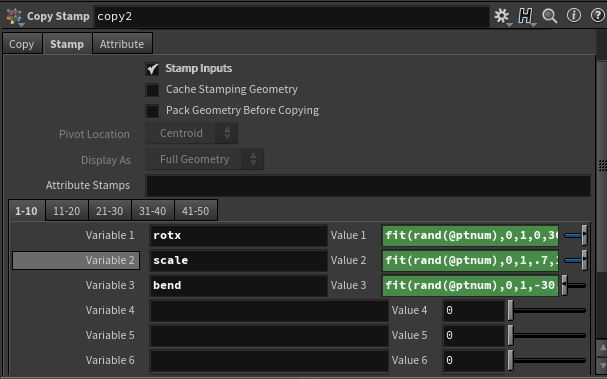
\includegraphics[width=\textwidth]{graphics/copy_stamp.jpg}
			 \end{minipage} 
		\end{itemize}

		Mit der Switch Node kann nun zwischen den beiden Versionen frei gewählt werden. 
		Die Variable kann in den Parametern der vorher genannten Nodes über den angegebenen Namen referenziert werden. Durch das rand(@ptnum) wird eine zufällige Zahl für jeden Punkt generiert. Durch fit werden die Werte einem angegebenen Zahlenbereich zugeordnet. fit(n, oldmin, oldmax, newmin, newmax) wird verwendet um eine beliebige Zahl, in unserem Fall die Nummer des Punktes, aus einem Zahlenbereich einem anderen Bereich zuzuordnen. Am Schluss hängen wir eine Null-Node an. \\
		\includegraphics*[scale=0.3]{graphics/grass_final.jpg}
		\includegraphics*[scale=0.53]{graphics/grass_1.jpg}\\
		In dem wir alle Nodes in einem Subnet speichern, können wir von dort aus auf ausgewählte Parameter zugreifen und diese übersichtlich anpassen.\\
		\includegraphics*[width=\textwidth]{graphics/subnet.jpg}
	\end{enumerate}
	
	\subsection*{Schilfrohr:}
	Das Schilfrohr besteht aus drei Teilen: Die Blüte, der Stiel und eine Fläche um wie bei dem Gras mehrere Stiele zusammen zu setzen.
	\subsubsection*{Blüte:}
	Die Blüte besteht aus einer Polygon Tube, der Radius und die Höhe kann beliebig gesetzt werden, sollte aber im Verhältnis zum Stiel stehen. Ich habe mich für einen Radius von 0.037 und eine Höhe von 0.27 entschieden. Die End-Caps sind an. Damit die Blüte rund wird, habe ich die Columns relativ hoch, auf 12, gestellt.\\
	Anschließend werden die End Caps mit der Polybevel Node abgerundet. Ich habe die Distanz auf 0.044 und die Divisions auf 3 gesetzt. So erhalten wir eine TikTak ähnliche Form.\\ 
	Diese wird mit der Color Node braun gefärbt und anschließend mit einer Transform Node auf der y-Achse so weit nach oben geschoben, bis sie auf den Stiel passt. Ich fand den Wert 0.34 für mein Beispiel passend.\\ 
	Anschließend verwende ich die remesh Node, um danach mit der Mountain Node die Blüte etwas deformieren zu können. Ich wollte keine große Veränderung, sondern nur dass die Blüte etwas uneben wird. Daher habe ich die Werte mit einer height von 0.02 und einer Element Size von 0.0001 sehr niedrig gesetzt.\\ 
	Um dem Low Poly Stil gerecht zu werden, verwende ich zum Schluss eine normal Node, welche dafür sorgt, dass die Blüte eckiger aussieht.\\
	\begin{minipage}{0.5\textwidth}
		Das Network und die Blüte sehen dann in etwa so aus:
	\end{minipage}
	\begin{minipage}{0.5\textwidth}
		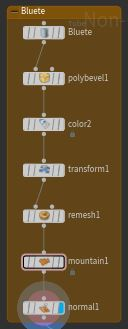
\includegraphics[width=0.28\textwidth]{graphics/bluete_node.jpg}
		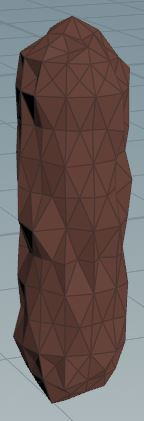
\includegraphics[width=0.25\textwidth]{graphics/bluete.jpg}
	\end{minipage}
	\subsubsection*{Stiel:}
	Der Aufbau des Stiels ist ähnlich dem der Blüte jedoch viel einfacher, er besteht nur aus einer Tube. Die Höhe habe ich auf 1 gesetzt und die Columns gerade so hoch, dass der Stiel rund wird. Die Anzahl der Rows habe ich relativ hoch, auf 41, gesetzt, damit später beim Biegen des Stiels gute Ergebnisse erzielt werden können. Anschließend habe ich den Stiel mit einer Color Node grün gefärbt.
	\subsubsection*{Zusammenfügen:}
	Als erstes wird die Blüte und der Stiel mit Hilfe einer boolean Node zu einem Objekt zusammengefügt, welches dann mit Bend gebogen werden kann. Der Winkel der Biegung wird, wie bei dem Gras, durch das Referenzieren eines Attributes in der Copy Stamp Node zufällig gesetzt. Das gleiche geschieht mit Hilfe einer Transform Node für die Größe der Stiele. Außerdem wird mit der Transform Node die Pflanze nach oben verschoben, bis sie auf dem Boden steht. Dies passiert prozedural, indem der y-Translate-Wert die Höhe des Stiels referenziert. So wird die Pflanze immer genau um die Hälfte der Höhe nach oben verschoben, und ist immer am Boden ausgerichtet, auch wenn sich die Höhe des Stiels ändert. \\
	\includegraphics*[width=0.8\textwidth]{graphics/stiel.jpg}\\
	Anschließend werden die Stiele, genau wie beim Gras, mit Zufallswerten auf Punkte übertragen. Diese wurden wieder mit Hilfe der Scatter Node aus einem Kreis extrahiert. Man kann mit dem Offset der Scatter Node herumspielen, bis man ein Ergebnis findet, das einem gefällt.\\
	Dies war mein Endergebnis: \\
	\includegraphics*[width=0.6\textwidth]{graphics/schilf.jpg}\\
	
	\subsection*{Blumen:}
	\subsubsection*{Blüte:}

	Um eine einfache Blüte zu machen, brauchen wir nur eins: ein Blatt. Um ein Blatt zu erstellen, brauchen wir erstmal zwei Linien. Line2(Direktion (0;0;1); Length 0.9; Points 8) bildet die Hauptader des Blattes. Ihr fügen wir die Attribute zum Verformen des Blattes wie z.b. die Rotation, Skalierung usw. mit Hilfe der Node Attribwrangle hinzu.
	\begin{itemize}
		\item f@np= @ptnum/(@numpt*1.0);     	 	-> np = aktuelle punkt / (anzahl pkt * 1.0)
		\item f@rot= chramp('rot',@np); 			-> erstellt ramp zur rotation (später bei Copy)
		\item f@sc = chramp('sc',@np);				-> erstellt ramp zur skalierung
		\item @pscale = @sc;					-> setzt skalierung = sc
		\item f@curve\_loc = chramp('curve\_loc',@np); 	-> curve loc ramp  (später bei Line1 und Copy)
		\item f@screw\_loc = chramp('screw\_loc',@np);	-> screw loc ramp
	\end{itemize}	
	\includegraphics*[scale=0.55]{graphics/blossom.JPG}
	\includegraphics*[scale=0.55]{graphics/wrangle.jpg}\\
	Durch sie können wir das Blatt nachher nach unseren Bedürfnissen anpassen und verformen, wodurch sich viele verschieden Blüten bilden lassen würden. In unserem Fall bleiben wir bei einem Design, da unser Stil LowPoly ist. Da es bei den Linien schwer ist zu erkennen wie das Blatt im Nachhinein aussehen wird, werden wir die Attribute erst später genauer setzen.\\ \\
	Line1(Direction(1;0;0); Length 0.46; Points 3) stellen die Nebenadern dar. Ihr geben wir mit Attribcreate ein weites Attribut namens curve\_loc\_to\_vop, dessen Betrag wir der später folgenden Copy Node entnehmen und daher erst später setzen. Die Linie hat später einen Knick, wodurch sich eine Delle im Blatt bildet.\\ \\
	Dieses Attribut bearbeiten wir mit AttribVOP um die Werte der Position des Knicks anzupassen. Dazu nehmen wir die Position des Punktes und lassen x und z unberührt. y berechnen wir neu. Dazu nehmen wir den aktuellen punkt (ptnum), wandeln ihn zu einem float um (inttofloat) und teilen (divide) ihn durch die Anzahl der Punkte (numpt), welche durch (divconst) 1.192 geteilt wurde. Das Ergebnis geht in eine Ramp (Ramp) und wird anschließend mit dem Attribut curve\_loc\_to\_cop (bind) multipliziert. Durch verändern der Konstanten verändert sich der dadurch entstandene Knick.\\ 
	\includegraphics*[width=\textwidth]{graphics/attribvop.JPG}\\
	\begin{minipage}{0.3\textwidth}
		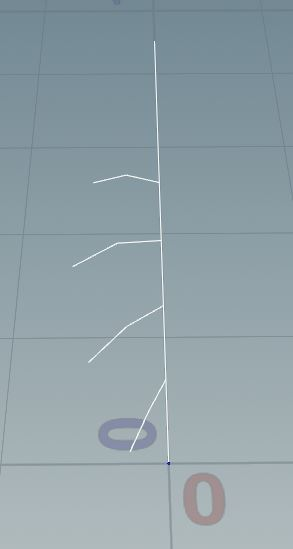
\includegraphics[width=0.7\textwidth]{graphics/blossom1.JPG}
	\end{minipage}
	\begin{minipage}{0.7\textwidth}
		Anschließend nutzen wir copy um Line1 an die Punkte der Line2 zu setzen. Hier legen wir jetzt unter Stamp die bereits erwähnte curve\_loc Variable (Variable:c\_loc; Value:@curve\_loc) an. Die Linien lassen wir dazu noch rotieren um eben die Form eines Blattes zu bekommen. Dazu geben wir unter Copy dem y Wert von Rotate den Wert "fit01(@rot,90,-90)". Fertig is das Skelett des Blattes.
	\end{minipage}

	\begin{minipage}{0.5\textwidth}
	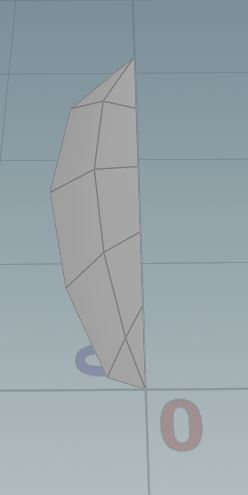
\includegraphics[width=0.3\textwidth]{graphics/blossom2.JPG}
	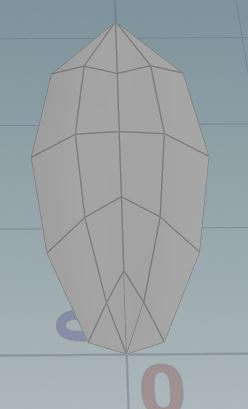
\includegraphics[width=0.35\textwidth]{graphics/blossom3.JPG}
	\end{minipage}
	\begin{minipage}{0.5\textwidth}
		Um es jetzt zu einem Blatt zu machen, legen wir eine Haut (skin) drüber und spiegeln (mirror) es. Jetzt können wir zurück zu attribVOP gehe und die Ramps nach Belieben ändern. Optional kann das Blatt noch etwas gebogen (bend (Bend -53.8)) werden.
	\end{minipage}
	
	Jetzt muss das Blatt nur noch in einem Kreis positioniert werden und fertig ist die Blüte.\\
	Dazu geben wir dem Blatt noch eine Transform Node mit, in der wir bei Rotate y den Wert 'point('../foreach\_begin', 0, 'roff', 0)' geben. Auf den greifen wir gleich innerhalb der Schleife zu, um die Blätter mit zu rotieren.
	Als erstes erstellen wir eine For Each Schleife. In begin kommt ein attribwrangle.
	\begin{lstlisting}[basicstyle=\scriptsize]
		int pnt = addpoint(0, {0,0,0});
		float roff = chf('Angle') * @elemnum;
		setpointattrib(0, 'roff', pnt, roff, 'set');
	\end{lstlisting} 
	Wir legen also Punkte an, die alle bei 0,0,0 liegen an die die Blätter gesetzt werden, aber lassen das Blatt bei jedem Punkt rotieren (roff). Oberhalb gibt Number count (9) an, wie viele Blütenblätter erstellt werden. Unterhalb kann man mit Angle (160) den Winkel anpassen. Wenn man mehr oder weniger Blüten Blätter haben will, muss man den Winkel immer wieder neu anpassen.\\ 
	Zwischen Begin und End kommt nun ein copy to points, dessen erster Input unser Blatt, zweiter Input Begin und output End ist. Dadurch wird an jeden Punkt ein Blütenblatt kopiert und dessen Rotation gesetzt. 
	Zum Abschluss setzen wir eine Null Node die wir BLOSSOM\_OUT nennen, um später einfacher auf die Blüte zugreifen zu können. Fertig ist unsere Blüte.\\
	\includegraphics*[scale=0.45]{graphics/blossom4.JPG}
	
	\subsubsection*{Blatt:}
	Das Blatt könnte man jetzt auf dieselbe weise wie das Blüten Blatt machen, da die Blätter am Stängel aber weniger wichtiger sind, gestalten wir dies etwas einfacher. Dazu nutzen wir L-Systeme.\\
	\begin{minipage}{0.3\textwidth}
		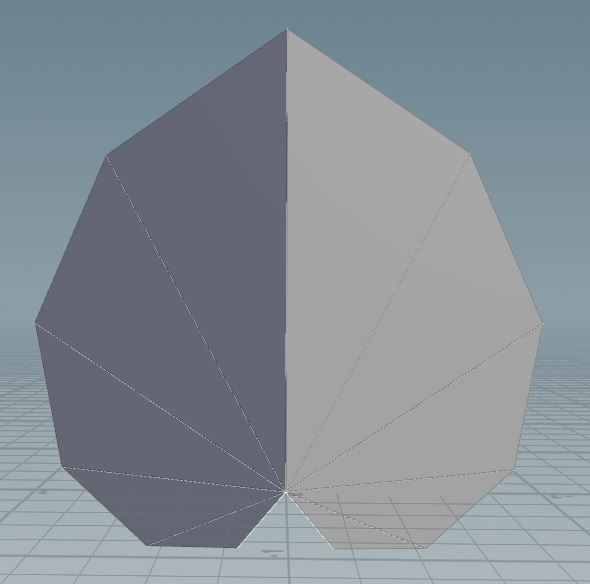
\includegraphics[width=0.9\textwidth]{graphics/leaf1.JPG}
	\end{minipage}
	\begin{minipage}{0.7\textwidth}
		\begin{lstlisting}[basicstyle=\scriptsize]
		Premise [A][B]
		Rule 1 A=[+A{.].C.}
		Rule 2 B=[-B{.].C.}
		Rule 3 C=FFFC
	\end{lstlisting} 
	Dazu erstellen wir Polygone (geometrische Figuren). Später Innerhalb der Blume verformen wir das Blatt, um es natürlicher aussehen zu lassen.\\
	Am Ende erstellen wir wieder eine Null Node LEAF\_OUT.
	\end{minipage}
	
	\subsubsection*{Kern:}
	Da wir uns ja im LowPoly befinden, habe ich anstatt der größeren Anzahl an Kernen nur eine Sphere genommen, diese etwas verkleinert (Uniform Scale 0.2), gestaucht (Radius(0;0.4;0)) und später innerhalb der Blume braun gefärbt. Den Schluss bildet wieder eine Null Node KERNEL\_OUT.\\
	Wenn man aber die Blume detaillierter darstellen möchte, sollte man auf die Anordnung der Kerner, welche sich Phyllotaxis nennt, achten. Diese bezieht sich auch auf die Blüten Blätter. 
	\begin{lstlisting}[basicstyle=\scriptsize]
		int num = chf("num");
		float phi = (1 *sqrt(5) / 2.0;
		float ang = 2* \$PI * (phi - 1) /phi;
		
		for(int i=0; i<num; i++)
		{
			float rad = i;
			vector pos = 
				set(cos(ang*i)*rad,0,sin(ang*1)*rad;
			int pt = addpoint(0, pos);
		}	
	\end{lstlisting} 
	\subsubsection*{Blume:}
	\begin{minipage}{0.5\textwidth}
		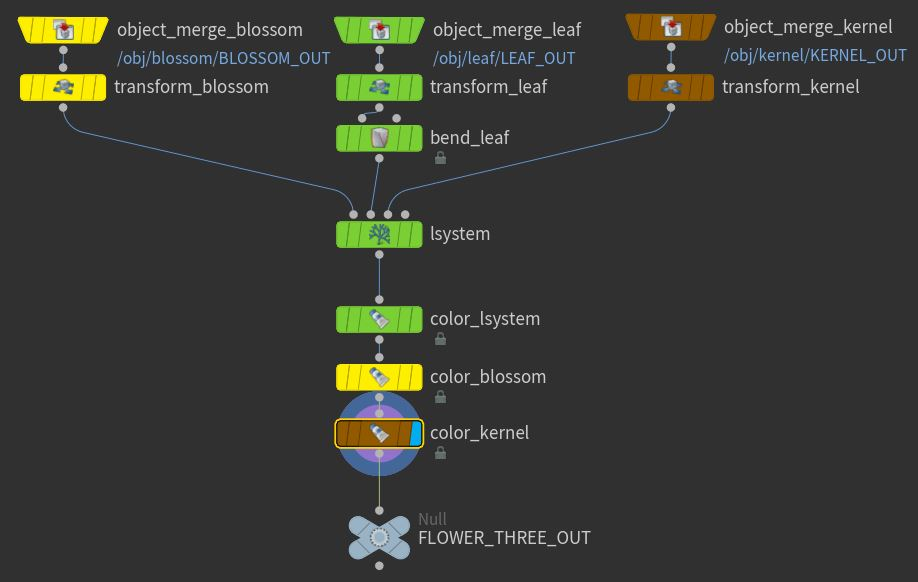
\includegraphics[width=0.98\textwidth]{graphics/flower_three.JPG}
	\end{minipage}
	\begin{minipage}{0.5\textwidth}
		Jetzt brauchen wir nur noch alles zusammenzufügen und unsere L-Systeme zu erstellen. 
		Um auf unsere Objekte zuzugreifen nutzen wir Object Merge. Dazu geben wir ihm unter Object1 jeweils eine Null Node. Jedem Object Merge hab ich jeweils noch ein Transform angehängt, um die einzelne Objekte anpassen zu können. Dem Blatt hab ich zusätzlich noch ein bend(Bend 22.5; Twist 55) gegeben, um es natürlicher wirken zu lassen.
		Die Objekte bilden den Input für unsere L Systeme (J = Blüte; K = Blatt; M = Kern)
	\end{minipage}

	\begin{minipage}{0.3\textwidth}
		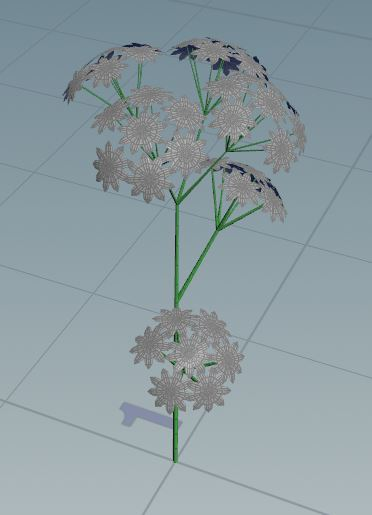
\includegraphics[width=0.8\textwidth]{graphics/flowerone1.JPG}
	\end{minipage}
	\begin{minipage}{0.7\textwidth}
	\begin{lstlisting}[caption={Flower One},basicstyle=\scriptsize]
		Premise !F(0.07)[B]!F(0.07)[E]!F(0.07)A
		Rule 1	A=!\\"[B]///[B]///[B]///[B]
		Rule 2	B=!-(20)\&F(0.05)C
		Rule 3	C=!\\"[D]//[D]//[D]//[D]//[D]//[D]F(0.04)J
		Rule 4	D=!-(20)\&F(0.04)J
		Rule 5	E=!-(20)\^F(0.05)C
	\end{lstlisting} 
	\end{minipage}
	\begin{minipage}{0.3\textwidth}
		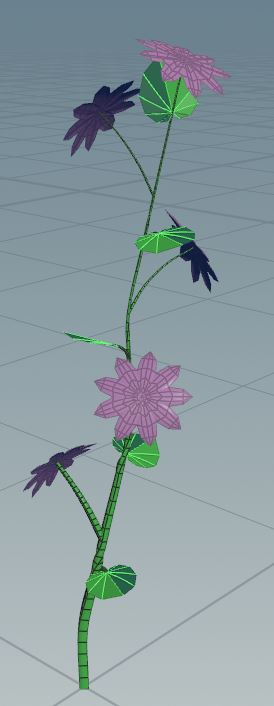
\includegraphics[width=0.7\textwidth]{graphics/flowertwo1.JPG}
	\end{minipage}
	\begin{minipage}{0.7\textwidth}
	\begin{lstlisting}[caption={Flower Two},basicstyle=\scriptsize]
		Premise F(0.05)A
		Rule 1	A = -(15)!F(0.05)[\^BBBBK]/(120)!F(0.03)[\^CCCJM]A
		Rule 2	B = -(20)!\&(10)F(0.004)
		Rule 3	C = -(10)!\^(10)F(0.02)
		Rule 4	D = -(15)!F(0.05)[\^BBBBK]/(120)[\^CCCJ]A
	\end{lstlisting} 
	Bei der zweiten Blume bildete sich ein Problem. Sie besteht aus Iterationen, wodurch man durch Verändern der Anzahl der Generationen ein Wachstum sehen kann. Das Problem: die Objekte bilden sich sofort, wodurch es zu einem unschönen Bild wurde. Das neue Blatt und die Blüte hängen ineinander. Durch einfügen einer Linie (Regel A; F(0.03)) sieht es aber akzeptabel aus.
	\end{minipage}
	\begin{minipage}{0.3\textwidth}
		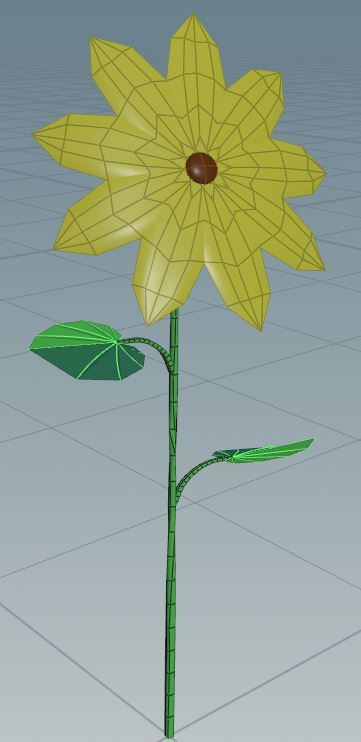
\includegraphics[width=0.7\textwidth]{graphics/flowerthree1.JPG}
	\end{minipage}
	\begin{minipage}{0.7\textwidth}
	\begin{lstlisting}[caption={Flower Three},basicstyle=\scriptsize]
		Premise !/(395)F!/(100)F[CCCK]/(196)F[CCCK]!/(183)F[AAAMJ]
		Rule 1	A = -(20)!F(0.02)
		Rule 2	B = -(20)!\^(20)F(0.02)
		Rule 3	C = -(20)!\&(20)F(0.02)
	\end{lstlisting} 
	\end{minipage}
		\begin{minipage}{0.3\textwidth}
		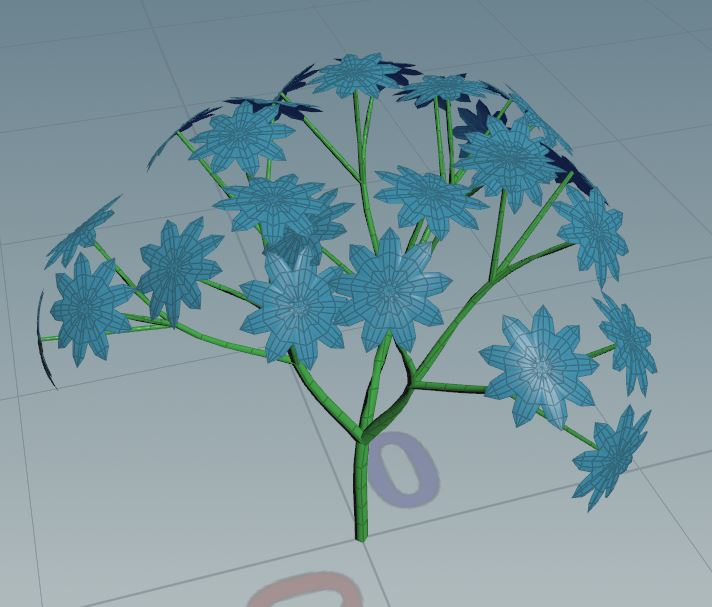
\includegraphics[width=0.9\textwidth]{graphics/flowerfour1.JPG}
	\end{minipage}
	\begin{minipage}{0.7\textwidth}
		\begin{lstlisting}[caption={Flower Four},basicstyle=\scriptsize]
			Premise FA
			Rule 1	A=!"[B]////[B]////BJ
			Rule 2	B=!\&FA
		\end{lstlisting} 
	\end{minipage}
	Mit Hilfe von Gruppen können wir die Blume nun einfärben (color). Erstmal färben wir alles Grün (\#21FF26), ohne eine Gruppe anzugeben. Die Blüte und den Kern färben wir durch Angeben der Gruppen lsysX, wobei X der jeweilige Input steht (Blüte = J; Kern = M). An Ende wie immer unser Null Node FLOWER\_OUT.
	
	\subsection*{Bäume:}
	\includegraphics*[scale=0.6]{graphics/Ali1.png}
	\includegraphics*[scale=0.9]{graphics/Ali2.png}
	\subsubsection*{Aufbau:} 
	\begin{minipage}{0.3\textwidth}
		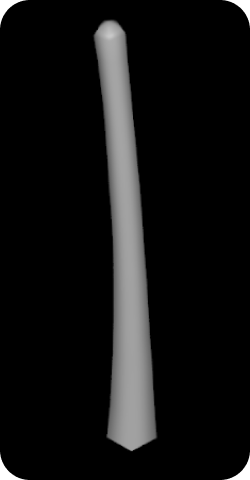
\includegraphics[width=0.8\textwidth]{graphics/Ali3.png}
	\end{minipage}
	\begin{minipage}{0.7\textwidth}
	Wir haben uns für den Low Poly Stil entschieden. Deswegen versuchen wir den Baum so simple wie möglich zu erstellen. Am Anfang benötigt man den Tree\_Trunk\_Generator um den Stamm vom Baum zu erstellen. Ich habe mich bei dem Radius für 1.5 und bei der Länge für 20 entschieden. Wenn man den Stamm biegen möchte, kann man dies bei 'Tropism' tun. Den Bend Wert, also wie stark der Stamm gebogen sein soll, habe ich auf 10 gesetzt.  Da es nach Low Poly aussehen soll, muss man bei 'Resolution' die Resolution und die Anzahl der divisions runter stellen, damit der Stamm weniger Ecken hat, an denen er gebogen werden kann. Dadurch wird das Ergebnis 'kantiger'.
	\end{minipage}
	\begin{minipage}{0.3\textwidth}
	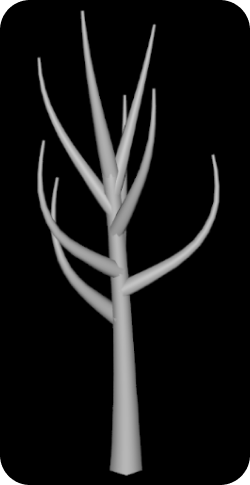
\includegraphics[width=0.8\textwidth]{graphics/Ali4.png}
	\end{minipage}
	\begin{minipage}{0.7\textwidth}
	Wir haben jetzt den Baumstamm fertig, und benötigen nun die Äste. Dies kann man mit der Node 'Tree\_Branch\_Generator' erledigen. Die Anzahl der Ästen habe ich auf 8 gesetzt und die Länge auf 0.7. Aber damit die Äste nicht gerade werden, muss man in 'Tropism' bei 'Phototropism' die Gravitation einstellen. In diesem Fall habe ich bei 'Strength' eine positive Zahl (0.11) eingegeben, damit alle Äste nach oben zeigen. Man kann auch eine negative Zahl eingeben, wenn man möchte, dass sie nach unten zeigen. 
	\end{minipage}
	\begin{minipage}{0.3\textwidth}
	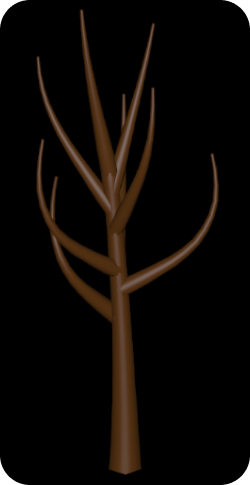
\includegraphics[width=0.8\textwidth]{graphics/Ali5.png}
	\end{minipage}
	\begin{minipage}{0.7\textwidth}
	Nun wird der Baum mit der Color Node eingefärbt, damit er nicht weiß bleibt. Ich habe mich für ein Braun mit dem Hex-Code: 351001 entschieden.
	\end{minipage}
	\begin{minipage}{0.3\textwidth}
		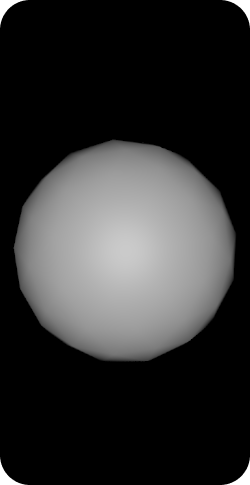
\includegraphics[width=0.8\textwidth]{graphics/Ali6.png}
	\end{minipage}
	\begin{minipage}{0.7\textwidth}
	Jetzt braucht man eine Sphere Node für die Blätter. Houdini hat auch ein normales Blatt das man benutzen kann. Aber anstatt dies zu benutzen, benutzen wir eine Sphäre, damit der Baum Low Poly artig aussehen wird. In der Node setzen wir den Primitive-type auf 'Polygon'. Dies teilt die Sphäre in mehrere Dreiecke, deren Anzahl man bei Frequency einstellen kann. Ich habe die Frequency zum Beispiel auf 3 gestellt, damit es nicht zu viele und nicht zu wenige werden. Um später, wenn alles zusammen gebaut wird, die Größe einstellen zu können, habe ich eine Transform Node hinzugefügt.
	\end{minipage}
	\begin{minipage}{0.3\textwidth}
		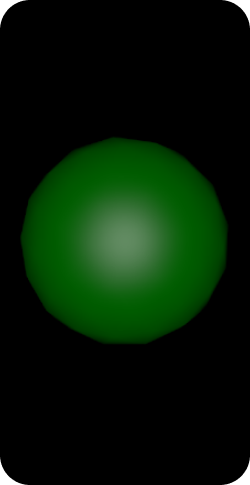
\includegraphics[width=0.8\textwidth]{graphics/Ali7.png}
	\end{minipage}
	\begin{minipage}{0.7\textwidth}
	Wie am Anfang wird hier eine Color Node gebraucht, damit die Blätter grün aussehen. Hex Code: 004B00
	\end{minipage}
	\begin{minipage}{0.3\textwidth}
		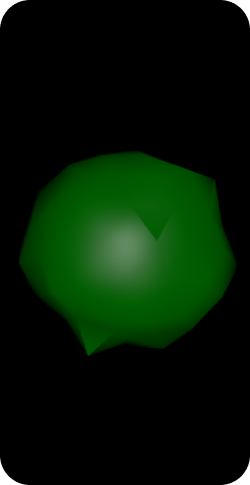
\includegraphics[width=0.8\textwidth]{graphics/Ali8.png}
	\end{minipage}
	\begin{minipage}{0.7\textwidth}
	Danach wird eine Mountain Node über die Sphere gelegt, um es natürlicher aussehen zu lassen. Ich habe folgende Werte gesetzt: 
	\begin{itemize}
		\item height: 7.28
		\item element size: 5.23
		\item Noise Type: Perlin
		\item Factal Type: Terrain
		\item Max Octaves:9
		\item roughness: 0.741
	\end{itemize}
	\end{minipage}
	\begin{minipage}{0.3\textwidth}
		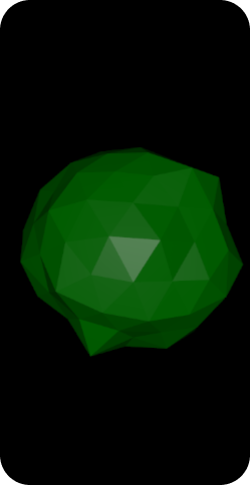
\includegraphics[width=0.8\textwidth]{graphics/Ali9.png}
	\end{minipage}
	\begin{minipage}{0.7\textwidth}
		Dann wird die Edgecusp Node angwendet damit es mehr nach Low Poly aussieht.
	\end{minipage}
	\begin{minipage}{0.3\textwidth}
		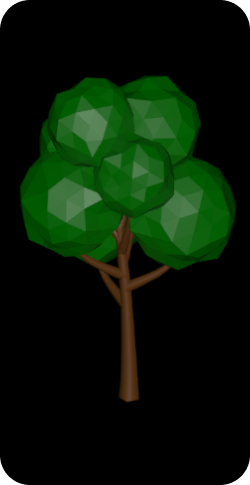
\includegraphics[width=0.8\textwidth]{graphics/Ali10.png}
	\end{minipage}
	\begin{minipage}{0.7\textwidth}
		Letztendlich wenden wir die Tree\_Leaf\_Generator Node an. Hier kann man einstellen wie viele Blätter man haben möchte und wo sie plaziert sein sollen. Da wir eine Sphäre für mehrere Blätter haben, sollte man die 'Leaf Node Distance' ziemlich weit auseinander einstellen (bei mir auf 5) damit pro Ast nur eine Sphäre daraufgesetzt wird. Bei 'Size Ramp' stellt man auch ein wo sich die Blätter auf den Ästen befinden sollen. Diese habe ich weit nach rechts gesetzt, damit die Sphäre am Ende der Äste sind.
	\end{minipage}
	Der ganze Aufbau des Low Poly Baums sieht mit den Nodes folgendermaßen aus:\\
	\includegraphics*[width=0.6\textwidth]{graphics/Ali11.png}
\end{document}